\documentclass[notitlepage,letterpaper,12pt]{article} % para articulo

% Este es un comentario <- Los comentarios comienzan con % 
% todo lo que se escriba hasta el final de la linea será ignorado <- Este es otro comentario

%Lenguaje del documento
\usepackage[spanish]{babel} % silabea palabras castellanas <- Puedo poner comentarios para explicar de que va este comando en la misma línea

%Encoding
\usepackage[utf8]{inputenc} % Acepta caracteres en castellano
\usepackage[T1]{fontenc} % Encoding de salida al pdf

%Paquetes mara mayor comodidad
\usepackage[normalem]{ulem}
\providecommand{\e}[1]{\ensuremath{\times 10^{#1}}}
\usepackage{aas_macros}

\usepackage{textcomp}
\usepackage{gensymb}


%Hipertexto
\usepackage[colorlinks=true,urlcolor=blue,linkcolor=blue]{hyperref} % navega por el doc: hipertexto y links

%Aquello de las urls
\usepackage{url} 

%simbolos matemáticos
\usepackage{amsmath}
\usepackage{amsfonts}
\usepackage{amssymb}
\usepackage{physics} 

% permite insertar gráficos, imágenes y figuras, en pdf o en eps
\usepackage{graphicx}
\usepackage{epstopdf}
\usepackage{multirow}
\usepackage{float}
\usepackage[export]{adjustbox}
% geometría del documento, encabezados y pies de páginas, márgenes
\usepackage{geometry}
\usepackage{comment}
\geometry{letterpaper}       % ... o a4paper o a5paper o ... 

\usepackage{natbib}


\usepackage{fancyhdr} % encabezados y pies de pg
\pagestyle{fancy}
\chead{\bfseries {}}
\lhead{} % si se omite coloca el nombre de la seccion
%\rhead{fecha del doc}
\lfoot{\it Informe Semana 5.}
\cfoot{ }
\rfoot{Universidad de los Andes}
%\rfoot{\thepage}
%margenes
\voffset = -0.25in
\textheight = 8.0in
\textwidth = 6.5in
\oddsidemargin = 0.in
\headheight = 20pt
\headwidth = 6.5in
\renewcommand{\headrulewidth}{0.5pt}
\renewcommand{\footrulewidth}{0,5pt}

\begin{document}
\title{Informe para Jaime: semana 6}
\author{
\textbf{Javier Alejandro Acevedo Barroso\thanks{e-mail: \texttt{ja.acevedo12@uniandes.edu.co}}}\\
\textit{Universidad de los Andes, Bogotá, Colombia}\\
} % Hasta aquí llega el bloque "author" (son dos autores por informe, orden alfabético)

%\date{Versión $\alpha \beta$ fecha del documento}
\maketitle %Genera el título del documento


%Resumen

%\begin{abstract}

%Usando un generador de señales 	CFG253 como fuente de voltaje en el circuito requerido de la practica, se observo la señal que produce un circuito RLC en un osciloscopio, con el objetivo de estudiar su resonancia eléctrica mediante la curva generada a partir de graficar el voltaje en la resistencia vs la frecuencia de oscilacion dada por la fuente  


 
%\end{abstract}

%Introducción
\section{Objetivos semanales}
\begin{enumerate}
\item Implementar test de masa y energía.
\item Hacer prueba de inestabilidad de Jeans con un $\bar{\rho}$ sin estar definido por $T = (G \bar{\rho})^{-1/2}$


\end{enumerate}

\section{Test de masa y energía}
Se rastreó la evolución temporal de la masa total en el sistema definida por:
\begin{equation}
M(t) = \sum_{X_\text{min}}^{X_\text{max}} \sum_{V_\text{min}}^{V_\text{max}} f(x,v,t) \Delta v \Delta x.
\end{equation}
A partir de ahí, se calculó el cambio en la masa a través de: 
\begin{equation}
\delta M = \frac{M(t) - M(0)}{M(0)}.
\end{equation}

La evolución del $\delta M$ fue cero completo  en todos los instantes.

Para la energía, se calculó la energía cinética total del sistema $K(t)$ como :
\begin{equation}
K(t) = \frac{1}{2} \sum_{X_\text{min}}^{X_\text{max}} \sum_{V_\text{min}}^{V_\text{max}} f(x,v,t) v^2 \Delta v \Delta x,
\end{equation}
y la energía potencial $U(t)$ como:
\begin{equation}
U(t) = \frac{1}{2} \sum_{X_\text{min}}^{X_\text{max}} \rho(x) \phi(x) \Delta x.
\end{equation}



A continuación se presenta la evolución temporal de la energía potencial, cinética, la energía total, y la diferencia entre energía potencial y cinética. 


\begin{figure}[h]
  \centering
   \includegraphics[scale= 0.8]{sadGraph0.png}
  \label{sadGraph0}
\end{figure}

La línea negra representa la energía inicial del sistema.

A continuación se presenta la misma gráfica, pero fijando la energía potencial inicial en cero.

\begin{figure}[h]
  \centering
   \includegraphics[scale= 0.8]{sadGraph.png}
  \label{sadGraph}
\end{figure}

\newpage

\section{Fijar $\bar{\rho}$}
Recapitulando, $T = (\bar{\rho} G)^{-1/2}$ y hasta ahora siempre había fijado $V = L/T$, donde $V$ se usa para definir el dominio del espacio de fase.

Corrí la simulación con $V = 2$, $L = 1$, $T =1$, la densidad promedio sería $\bar{\rho} = 1/(G T^2) = 4$ 
No se logró observar la inestabilidad de Jeans.


Corrí la simulación con $V = 2$, $L = 1$, $T =1$ y $\bar{\rho}$ Siendo la mitad del calculado con $T$. 
No se logró observar la inestabilidad de Jeans.

Notando que en el paper \citet{2013ApJ...762..116Y} (figura 9) se habla de que la dinámica del sistema depende no solo del $\sigma$ de velocidad, sino de la relación $\sigma / \Delta v$, hice el experimento de duplicar la resolución del sistema, de forma que a pesar de reducir el $\bar{\rho}$ y la dispersión de velocidad $\sigma = \sqrt{\frac{4 \pi G \bar{\rho}}{k^2}}$, la relación $\sigma / \Delta v$ es en realidad mayor.
En este caso, se activó la inestabilidad de Jeans.

En la figura (9) del artículo se muestra que la evolución del coeficiente de Fourier termina estando determinada por $\sigma / \Delta v$.
Voy a intentar reproducirla en mi trabajo y llevarla a la reunión.

\bibliographystyle{unsrtnat} % estilo de las referencias 
\bibliography{bibTes.bib} %archivo con los datos de los artículos citados


%\bibliography{mybib.bib} %archivo con los datos de los artículos citados

% Forma Manual de hacer las referencias
% Se escribe todo a mano...
% Descomentar y jugar

%\begin{thebibliography}{99}
%\bibitem{Narasimhan1993}Narasimhan, M.N.L., (1993), \textit{Principles of
%Continuum Mechanics}, (John Willey, New York) p. 510.

%\bibitem{Demianski1985}Demia\'{n}ski M., (1985), \textit{Relativistic
%Astrophysics,} in International Series in Natural Philosophy, Vol 110, Edited
%by \textit{D. Ter Haar}, (Pergamon Press, Oxford).
%\end{thebibliography}
.
%Fin del documento
\end{document}


Así mismo, el factor de calidad $Q$ está dado por:
\begin{equation}
Q = \frac{1}{R} \sqrt\frac{L}{C}
\end{equation}
Por lo tanto, el valor del factor de calidad

%Todo lo que escriba aquí será ignorado, aunque no fuera un comentario...
\begin{table}[h!]
\centering
\begin{tabular}{|l|l|l|}
\hline
2 cm   & 4 cm   & 8 cm   \\ \hline
175,77 & 129,77 & 88,77  \\ \hline
223,77 & 129,77 & 114,77 \\ \hline
219,77 & 134,77 & 77,77  \\ \hline
190,77 & 120,77 & 83,77  \\ \hline
\end{tabular}
\caption{Número de colisiones a diferentes distancias en cinco minutos.}
\label{tiempoFijo}
\end{table}

\begin{figure}[h]
  \centering
   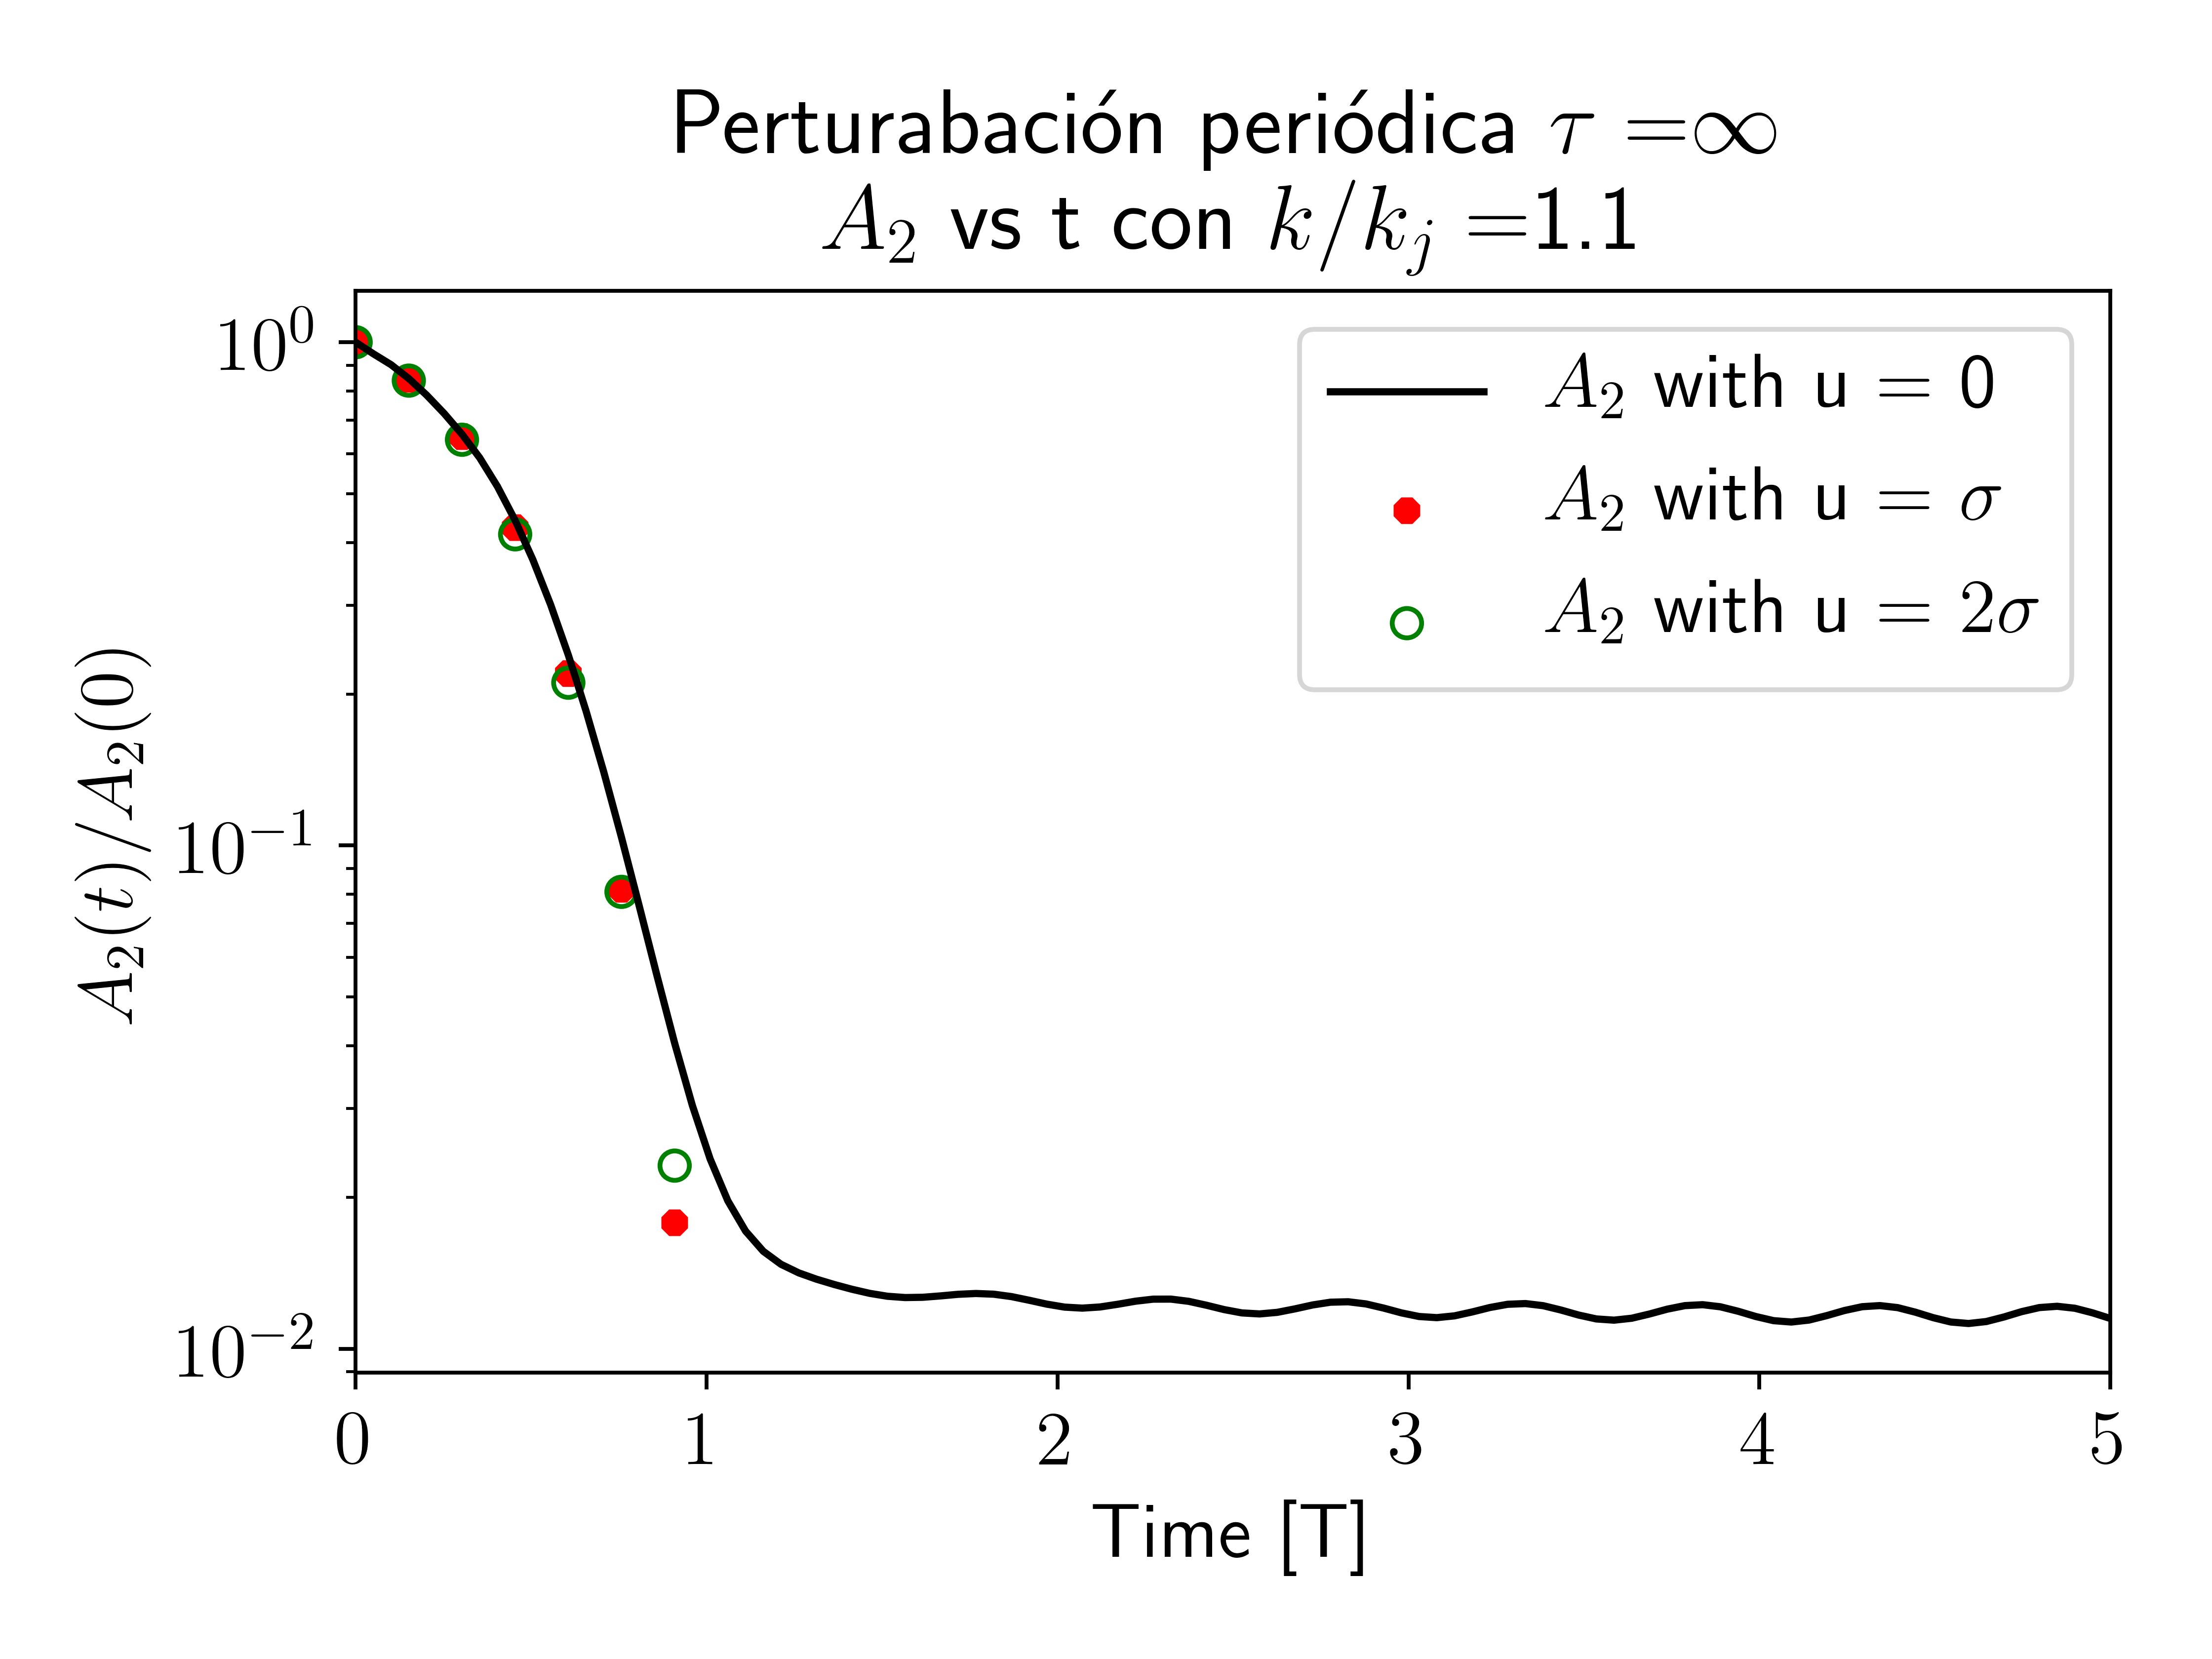
\includegraphics[scale= 0.8]{Jeans2Coef.png}

  \label{fig: cobre}
\end{figure}

\begin{figure}[h]
  \centering
   \includegraphics[scale= 0.8]{jairos.png}
  \caption{Gráfica del periodo de la pulsación para diferentes razones entre las frecuencias naturales utilizando una pesa de 200g. Es de resaltar que el pico no está centrado en 1 pero está bastante cerca. Esto probablemente se debe a errores a la hora de medir la longitud de los péndulos.}
  \label{fig: cobre}
\end{figure}
